
%
%	Calibration
%

\section{Calibration}\label{Section_Calibration}
\Headerfooter{Calibration}

\subsection{ID detector calibration}
\vs\hs ID detector calibration!

\begin{figure}[tbp]
	\centering
	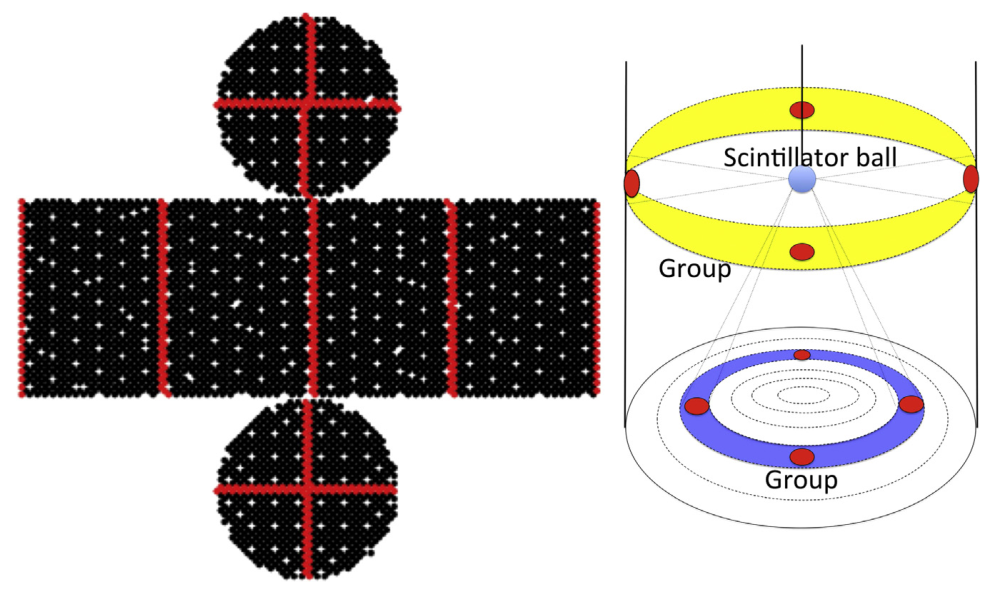
\includegraphics[width=10cm]{Figures/Calibration/CalibPMT}
	\caption[Location of standard PMTs in ID and schematic view of the groups of PMTs]{\label{Calibration_CalibPMT} Location of standard PMTs in ID (left) and schematic view of the groups of PMTs (right)~\cite{2014AbeCalib}.}
\end{figure}

\begin{figure}[tbp]
	\centering
	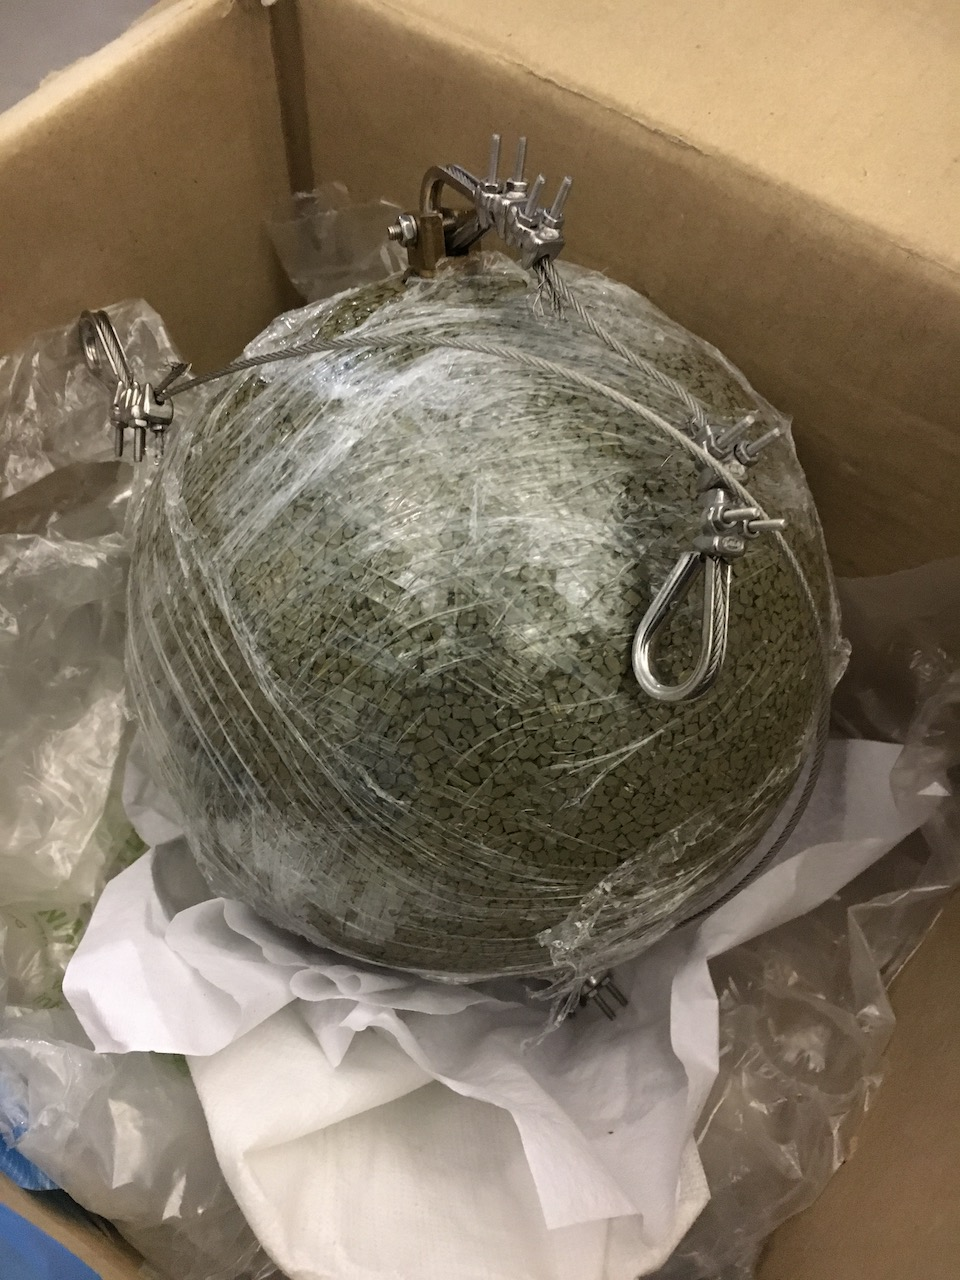
\includegraphics[width=6cm]{Figures/Calibration/Ni}
	\caption[Picture of the Ni-Cf source]{\label{Calibration_Ni} Picture of the Ni-Cf source.}
\end{figure}

\begin{figure}[tbp]
	\centering
	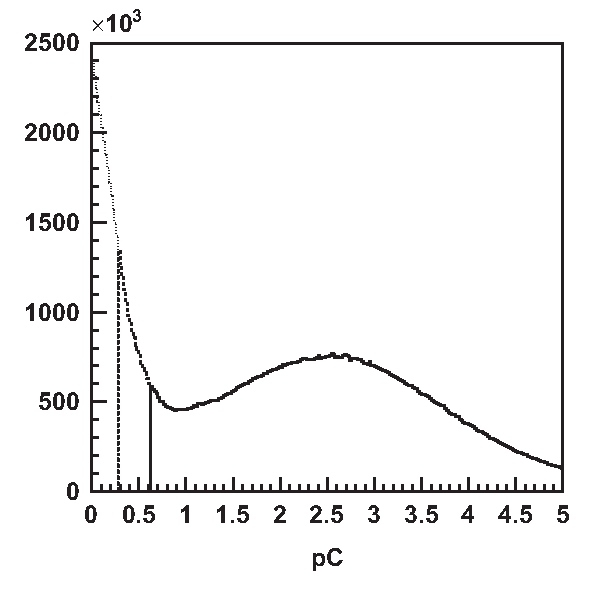
\includegraphics[width=8cm]{Figures/Calibration/Single-pe}
	\caption[Single-pe distribution of the Ni-Cf source data in SK-III]{\label{Calibration_Single-pe} Single-pe distribution of the Ni-Cf source data in SK-III~\cite{2014AbeCalib}. The dashed line shows the data with double gain and half threshold. The dotted line is linear extrapolation.}
\end{figure}

\begin{figure}[tbp]
	\centering
	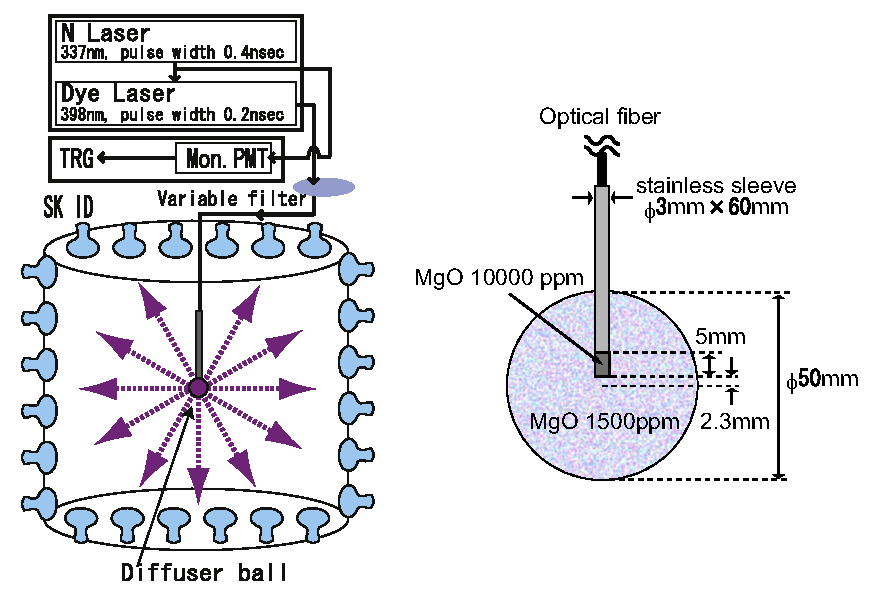
\includegraphics[width=10cm]{Figures/Calibration/TimingCalib}
	\caption[Schematic view of the timing calibration system and cross section of the diffuser ball]{\label{Calibration_TimingCalib} Schematic view of the timing calibration system (left) and cross section of the diffuser ball (right)~\cite{2014AbeCalib}.}
\end{figure}

\begin{figure}[tbp]
	\centering
	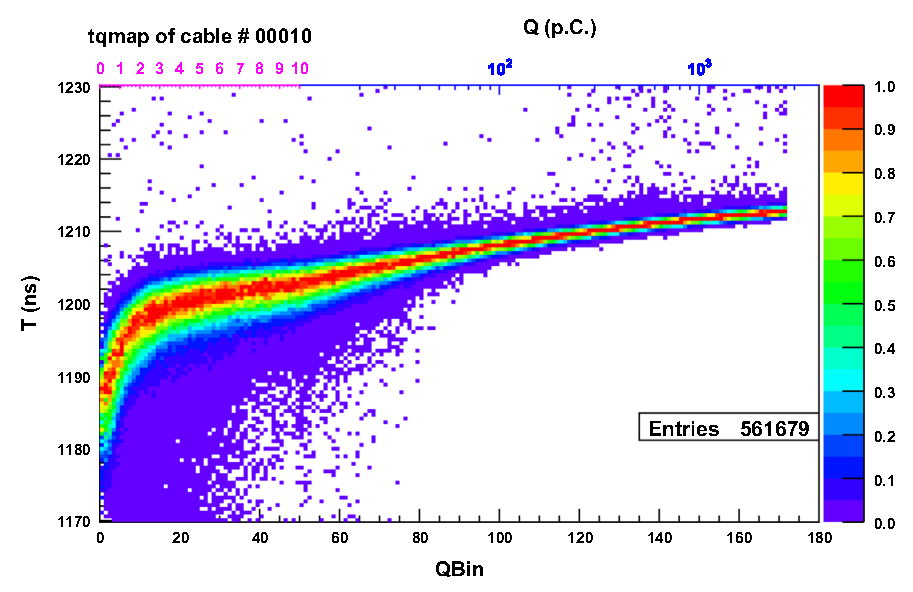
\includegraphics[width=10cm]{Figures/Calibration/TQ}
	\caption[Timing and charge distribution for a readout channel]{\label{Calibration_TQ} Timing and charge distribution for a readout channel~\cite{2014AbeCalib}. Horizontal axis shows charge (QBin) of each hit. Vertical axis shows TOF-corrected hit timing.}
\end{figure}

\begin{figure}[tbp]
	\centering
	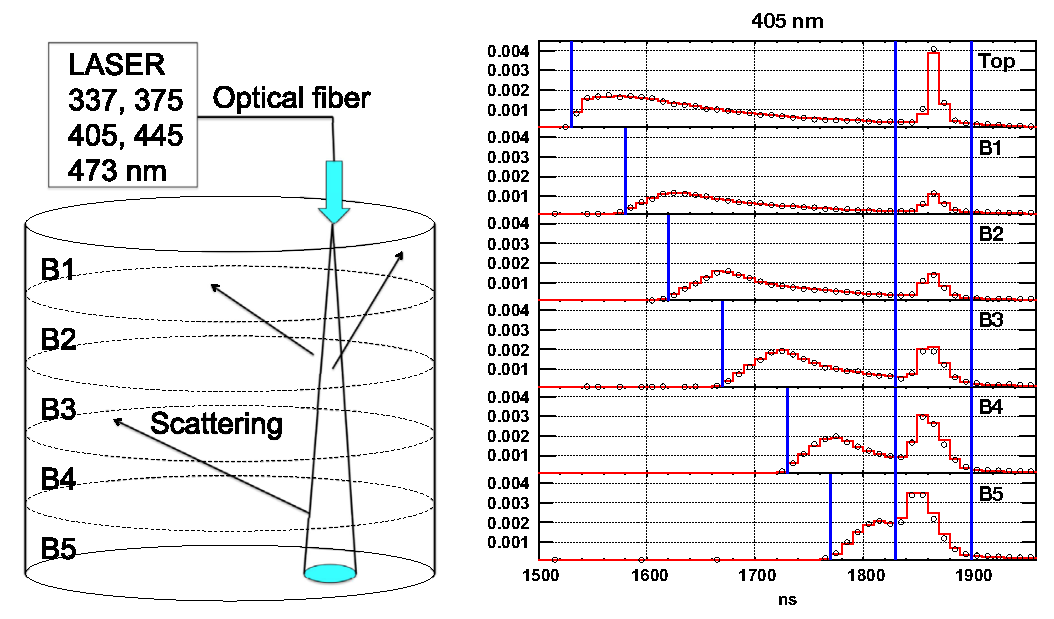
\includegraphics[width=12cm]{Figures/Calibration/LaserCalib}
	\caption[Schematic view of the laser calibration system and TOF-subtracted timing distributions of the laser calibration data and MC]{\label{Calibration_LaserCalib} Schematic view of the laser calibration system (left) and TOF-subtracted timing distributions of the laser calibration data and MC (right)~\cite{2014AbeCalib}. Water parameter tuning is performed using top PMTs that are 2 m away from the laser light injector, and barrel PMTs. Barrel is separated into five regions, from B1 to B5. B3 includes PMTs for 11 lines and the others include PMTs for 10 lines. In the left figure, the cyan shaded circle spot on the bottom shows the beam target used in the TOF calculation. In the right figure, the black circle shows data and the red histogram shows MC. Both data and MC are normalized by observed total photoelectrons. Time region between the left two blue solid vertical lines is used for the water parameter tuning. Right time region is used for the PMT reflectivity measurement.}
\end{figure}

\begin{figure}[tbp]
	\centering
	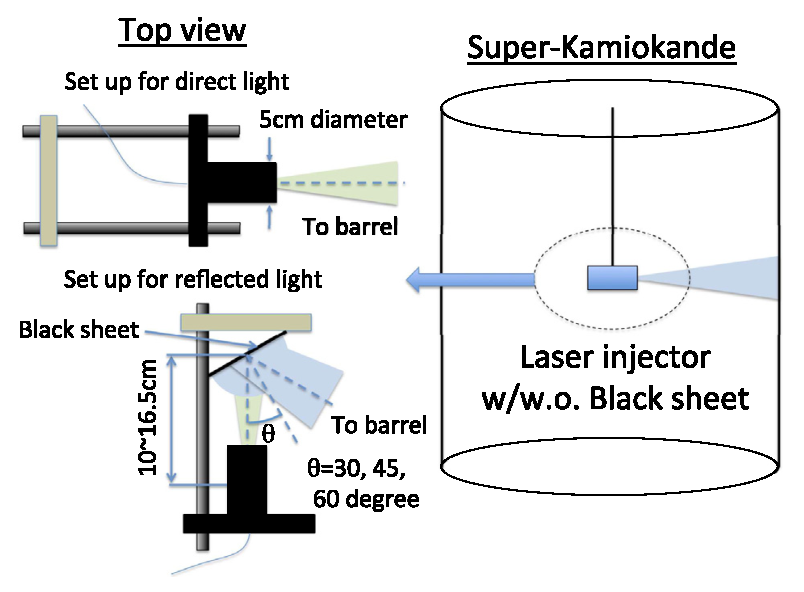
\includegraphics[width=10cm]{Figures/Calibration/CalibBS}
	\caption[Schematic view of the black sheet reflectivity measurement]{\label{Calibration_CalibBS} Schematic view of the black sheet reflectivity measurement~\cite{2014AbeCalib}. Left figure shows the top view. The laser light injector is inserted from the top center of the SK tank and the reflected light is measured by ID PMTs.}
\end{figure}

\newpage
